
\chapter{使用简介}
\label{chap:guide}

为方便使用及更好的展示~\LaTeX{}~排版的优秀特性,本人对模板的框架和文件体系进行了细致地处理,尽可能地对各个功能和板块进行了模块化和封装,对于初学者来说,众多的文件目录也许会让人觉得有些无所适从,但阅读完下面的使用说明后,您会发现原来使用思路是简单而清晰的,而且,当对~\LaTeX{}~ 有一定的认识和了解后,会发现其相对~Word~类排版系统的极具吸引力的优秀特性。所以,如果您是初学者,请不要退缩,请稍加尝试和坚持,让自己领略到~\LaTeX{}~的非凡魅力。 并可以通过阅读相关资料如~ \citep{wikibook2014latex}~ 来完善自己的使用知识。

\section{先试试效果}

ucasthesis~模板不仅只是提供了相应的类文件,同时也提供了包括参考文献等在内的完成学位论文的一切要素,所以,下载时,推荐下载整个~ucasthesis~文件夹,而不是单独的文档类。

下载~ucasthesis~文件夹并解压后,请在文件夹内找到~“Compile.bat”,双击运行,即可获得本说明文档,而这,也完成了学习使用此模板撰写论文的一半进程,什么?这就学成一半了,这么简单???,是的,就这么简单!

编译完成后,可以进入各个子目录逛逛,熟悉下模板框架。

\section{常见使用问题}

\begin{enumerate}
  \item 模板文档的编码为~utf-8~编码,若出现文本编辑器无法打开文档或打开文档乱码的问题,请检查您使用的编辑器对utf-8编码的支持,如果使用~WinEdit~作为文本编辑器,应在其

  “options --》 Preferences --》 wrapping”

  选项卡下将两种 “Wrapping Modes” 中的内容:

  “TeX;HTML;ANSI;ASCII|DTX...”

  修改为:

  “TeX;\textbf{UTF-8|ACP;}HTML;ANSI;ASCII|DTX...”

  同时,取消

  “options --》 Preferences --》 Unicode”

  中的“Enable ANSI Format...”选项。
\end{enumerate}

\section{各文档及目录简介}

\subsection{Thesis.tex文档 }

Thesis.tex文档为主文档,其设计和规划了论文的整体框架,通过对其的阅读可以让用户了解整个论文框架的搭建。

\subsection{Compile.bat}

%Compile.bat为编译此模板的Dos脚本,通过双击运行此脚本即可获得编译后的PDF文档,编译生成的文档及临时文件皆位于Tmp文件夹内。在此脚本中可以设定编译器为“pdflatex” or “xelatex” (default,且极力推荐使用xelatex 编译中文及中英文混排的\LaTeX{}文档)。
%
%若你倾向于使用WinEdit的编译方式,则请在 "Thesis.tex" 和 "Main\textunderscore Content.tex" 中为所有文件提供完整的搜索路径。 如 
%
%\verb+
\chapter{中国科学院大学学位论文撰写要求}
学位论文是研究生科研工作成果的集中体现,是评判学位申请者学术水平、授予其学位的主要依据,是科研领域重要的文献资料。根据《科学技术报告、学位论文和学术论文的编写格式》(GB/T 7713-1987)、《学位论文编写规则》(GB/T 7713.1-2006)和《文后参考文献著录规则》(GB7714—87)等国家有关标准,结合中国科学院大学(以下简称“国科大”)的实际情况,特制订本规定。

\section{学位论文的一般要求}

学位论文必须是一篇(或由一组论文组成的一篇)系统的、完整的学术论文。学位论文应是学位申请者本人在导师的指导下独立完成的研究成果,除论文中已经注明引用的内容外,不得抄袭和剽窃他人成果。对学位论文研究做出重要贡献的个人和集体,均应在文中以明确方式标明。学位论文的学术观点必须明确,且立论正确,推理严谨,数据可靠,层次分明,文字正确、语言通畅,表述清晰,图、表、公式、单位等符合规范要求。

\section{学位论文的水平要求}

硕士学位论文要选择在基础学科或应用学科中有价值的课题,对所研究的课题有新的见解,并能表明作者在本门学科上掌握了坚实的基础理论和系统的专门知识,具有从事科学研究工作或独立担负专门技术工作的能力。

博士学位论文要选择在国际上属于学科前沿的课题或对国家经济建设和社会发展有重要意义的课题,要突出论文在科学和专门技术上的创新性和先进性,并能表明作者在本门学科领域掌握了坚实宽广的基础理论和系统深入的专门知识,具有独立从事科学研究工作的能力。

\section{撰写学位论文的语言及文字}

除外国来华留学生及外语专业研究生外,研究生学位论文一般应采用国家正式公布实施的简化汉字撰写;应采用国家法定的计量单位。学位论文中采用的术语、符号、代号在全文中必须统一,并符合规范化的要求。

外国来华留学生可用中文或英文撰写学位论文,但须采用中文封面,且应有详细的中文摘要。外语专业的学位论文等应用所学专业相应的语言撰写,摘要应使用中文和所学专业相应的语言对照撰写。

为了便于国际合作与交流,学位论文亦可有英文或其它文字的副本。

\section{学位论文的主要组成部分}

学位论文一般由以下几个部分组成:中文封面、英文封面、致谢、中文摘要、英文摘要(Abstract)、目录、正文、参考文献、附录、作者简历及攻读学位期间发表的学术论文与研究成果。

\begin{enumerate}
  \item 学位论文题目应当简明扼要地概括和反映出论文的核心内容,一般不宜超过25个汉字(符),英文题目一般不应超过150个字母,必要时可加副标题。

  \item 论文摘要包括中文摘要和英文摘要(Abstract)两部分。论文摘要应概括地反映出本论文的主要内容,主要说明本论文的研究目的、内容、方法、成果和结论。要突出本论文的创造性成果或新见解,不宜使用公式、图表,不标注引用文献。英文摘要(Abstract)应与中文摘要内容相对应。摘要最后另起一行,注明本文的关键词(3-5个),关键词是为了文献标引工作从论文中选取出来,用以表示全文主题内容信息的单词或术语。

  \item 正文是学位论文的主体,包括引言(或绪论)、论文主体及结论等部分。
    \begin{itemize}
      \item 引言(或绪论)应包括选题的背景和意义,国内外相关研究成果述评,本论文所要解决的问题、所运用的主要理论和方法、基本思路和论文结构等。引言应独立成章,用足够的文字叙述,不与摘要雷同。

      \item 论文主体由于涉及不同的学科,在选题、研究方法、结果表达方式等有很大的差异,不作统一的规定。但必须严格遵循本学科国际通行的学术规范,言之成理,论据可靠,实事求是,合乎逻辑,层次分明,简练可读。

      \item 结论是对整个论文主要成果的总结,应明确、精炼、完整、准确。结论应明确指出本研究的创新点,对论文的学术价值和应用价值等加以预测和评价,说明研究中尚难解决的问题,并提出今后进一步在本研究方向进行研究工作的设想或建议。应严格区分本人研究成果与他人科研成果的界限。
    \end{itemize}

  \item 参考文献应本着严谨求实的科学态度,凡学位论文中有引用或参考、借用他人成果之处,均应按不同学科论文的引用规范,列于文末(通篇正文之后)。需正确区分直接引用和转引并明确加以标注。

  \item 学位论文印刷及装订要求:学位论文用A4标准纸打印、印刷或复印,按顺序装订成册。自中文摘要起双面印刷,之前部分单面印刷。论文必须用线装或热胶装订,不使用钉子装订。学位论文封面采用国科大统一规定的学位论文封面格式,封面用纸一般为150克(需保证论文封面印刷质量,字迹清晰、不脱落),博士学位论文封面颜色为红色,硕士学位论文封面颜色为蓝色。

  \item 学位论文的提交、保存与使用:学位申请者需按规定向国科大提交学位论文的印刷本和电子版,印刷本和电子版在内容与形式上应完全一致;国科大有权保存学位论文的印刷本和电子版,并提供目录检索与阅览服务,可以采用影印、缩印、数字化或其它复制手段保存学位论文;研究所、国科大有义务保护论文作者的知识产权。涉密学位论文在解密后,须按此规定执行。

  \item 本规定自印发之日起施行【2013年04月07日】,解释权属于校学位评定委员会,由国科大学位办公室负责解释。原《中国科学院研究生院研究生学位论文撰写规定》(院发学位字〔2012〕31号)同时废止。
\end{enumerate}
+ 
%
%应改为 
%
%\verb+\input{./Tex/Appeddix}+。

\subsection{Tmp文件夹}

运行编译脚本Compile.bat后,编译所生成的文档皆存于Tmp文件夹内,包括编译得到的pdf文档,其存在是为了保持工作空间的整洁,因为好的心情是很重要的.

\subsection{Style文件夹}

Style文件夹内包含有ucasthesis文档类的定义文件和配置文件,对于有特殊需求的用户,通过对它们的修改可以实现特定的类设定。

\begin{enumerate}
  \item ucasthesis.cls: 文档类定义文件,论文的最核心的格式即通过它来定义的。
  \item ucasthesis.cfg: 文档类配置文件,通过它设定论文的某些项目的显示内容,如“abstract”显示为“摘要”,“table of content”显示为“目~~~~录”而不是“目录”等(如果愿意,你也可以改过来)。
  \item commons.sty: 一些常用的文档设定, 如参考文献样式和文献引用样式等。
  \item custom.sty: 用户自定义命令的放置位置以及用来实现一些个性化设定,
\end{enumerate}

\subsection{Tex文件夹}

Tex文件夹内为论文的所有实体内容,正常情况下,这也是你\textbf{使用此模板撰写学文论文时,主要关注和修改的一个位置},详细分类介绍如下:

\begin{itemize}
  \item Frontpage.tex: 为论文封面内容, 及中英文摘要。
  \item Main\textunderscore Content.tex: 对需要出现的Chapter进行索引,开始写论文时,可以只索引当前章节,以便快速编译和查看,当最终所有章节完成后,再对所有章节进行索引即可。
  \item Chap\textunderscore XXXXX.tex: 为论文主体的各个章节,用户可根据需要添加和撰写,最终需要包含在论文中的章节,须在Main\textunderscore Content.tex中进行索引。
  \item Appendix.tex: 为附录内容
  \item Backmatter.tex: 为发表文章信息,致谢部分等。
\end{itemize}

\subsection{Img文件夹}

Img文件夹用于放置论文中所需要的图类文件,支持格式有:.jpg, .png, .pdf。其中,ucas.jpg为国科大校徽。

\subsection{Biblio文件夹}

Biblio文件夹内放置参考文献的索引信息文件:Myrefs.bib,此文件包含了需要引用的参考文献信息。

\section{数学公式、图片插入、参考文献等功能}

\subsection{数学公式}

常用数学公式的命令代码模板,请见如下WiKi:\url{http://zh.wikipedia.org/wiki/Help:%E6%95%B0%E5%AD%A6%E5%85%AC%E5%BC%8F}

\subsection{图片插入}

论文中图片的插入通常分为单图和多图,下面分别加以介绍:

\begin{table}
\centering
\caption{This is a table description that should be on top of the table 53252 3243242343243243242343242343243242343242343.}
\begin{tabular}{|c|c|c|}
    \hline 
    1 & 2 \\ \hline
    3 & 4 \\ \hline
\end{tabular}
\end{table}

单图插入:假设插入名为“ITC\textunderscore Q\textunderscore Criteria”(后缀可以为.jpg、.png、.pdf,下同)的图片,其效果如图\ref{fig:ITC_Q_Criteria},其命令可为:
\begin{verbatim}
\begin{figure}[!htbp]
  \centering
  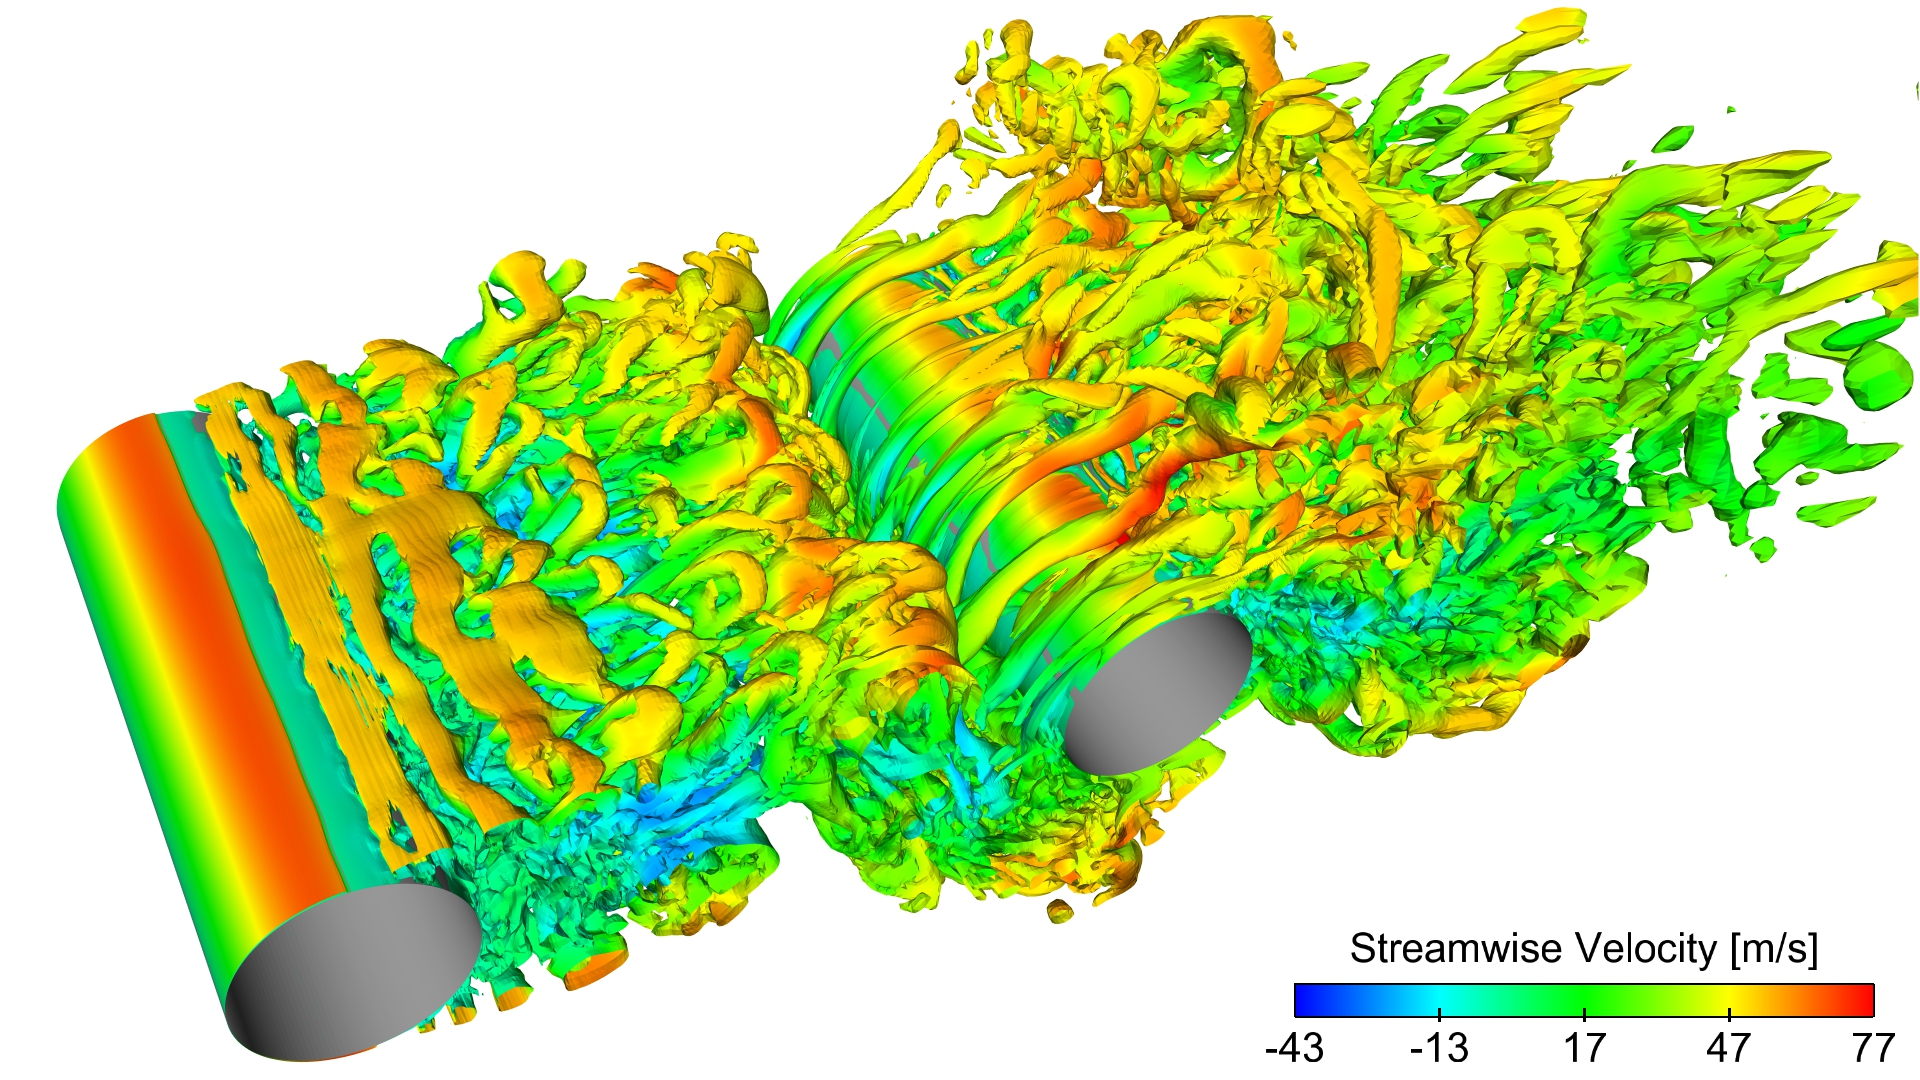
\includegraphics[width=\MyFactor\textwidth]{Img/ITC_Q_Criteria}
  \caption{Q判据等值面图}
  \label{fig:ITC_Q_Criteria}
\end{figure}
\end{verbatim}
\begin{figure}[!htbp]
  \centering
  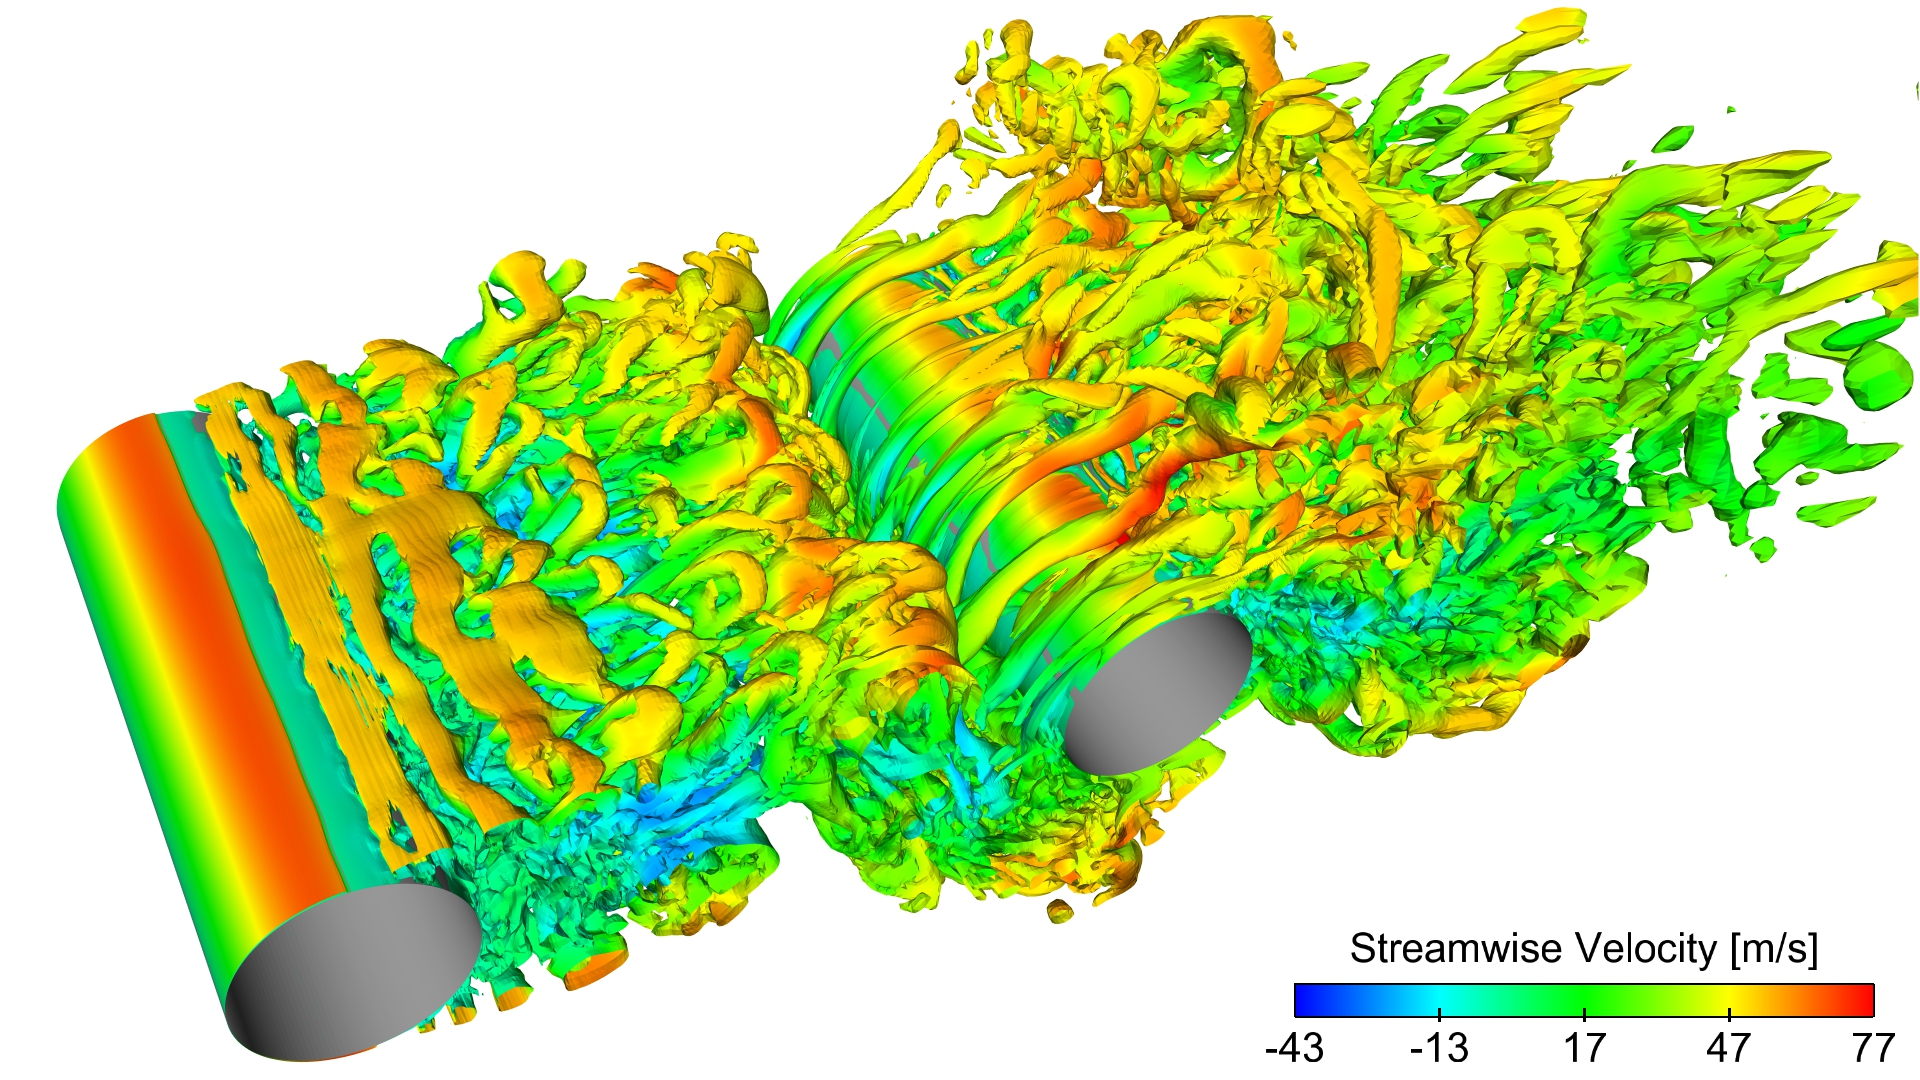
\includegraphics[width=\MyFactor\textwidth]{Img/ITC_Q_Criteria}
  \caption{Q判据等值面图}
  \label{fig:ITC_Q_Criteria}
\end{figure}



撰写论文中,插图和制表常用到的命令,已在\textbf{Useful Commands.txt}这个文本中给出了参考代码,大家只需copy使用即可。

\subsection{参考文献的使用}

参考文献的引用过程以实例的形式介绍,假设您需要引用名为“Document Preparation System”的文献,步骤如下:

1)使用“google scholar”搜索“Document Preparation System”,在目标条目下点击“引用”,展开后选择“ 导入BibTeX”,然后google将为你打开此文章的BibTeX索引信息,将它们copy添加到Myrefs.bib文件中(此文件位于“Biblio”文件夹下)。

2)你会发现索引信息中第一行为 “\verb|@article{lamport1986document,|”,其中的 
    
    "\verb|lamport1986document|" 
    
即为此文献的label,想要在论文中索引此文献,有两种索引模式:

textual mode, 输入:

“\verb|\citet{lamport1986document}|”

正如此处所示 \citet{lamport1986document}; 

parenthetical mode, 输入:

“\verb|\citep{lamport1986document}|

正如此处所示 \citep{lamport1986document}。

如此,即完成了文献的索引,请查看下本文档的“参考文献”一章,看看是不是就是这么简单呢?是的,就是这么简单!

不同的参考文献样式和文献引用样式可以通过在 "Thesis.tex" 中对 "commons.sty" 设置不同选项实现,如:

\verb+\usepackage[numbered]{commons}+ $\%$ default citation style. textual: Jones [1]; parenthetical: [1]

\verb+\usepackage[authoryear]{commons}+ $\%$ author year citation style. textual: Jones (1995); parenthetical: (Jones, 1995)

\verb+\usepackage[alpha]{commons}+ $\%$ alpha citation style. textual: not available; parenthetical: [Jon95]

参考文献索引更为详细的信息,请见\citep{wikibook2014latex}。
